\chapter{Синтез LQG}
\label{ch:chap3}
\section{Условие задачи}

Рассмотреть систему:
$$
    \begin{cases}
      \dot{x} = Ax + Bu + f \\
      y = Cx + Du + \xi
    \end{cases}, \tab x(0) = \begin{bmatrix}
      1 & 1 & 1 & 1
    \end{bmatrix}^T
$$ и в нашем случае $(f, \xi)$ - детерминированные гармонические сигналы, выполнить следующие шаги:
  \begin{itemize}
  \item  Проверить систему на стабилизируемость и обнаруживаемость
  \item  Построить схему моделирования системы, замкнутой регулятором, состоящем
  из наблюдателя состояния и закона управления и $u = Kx$.
  \item Задаться значениями пар матриц $(Q_K,R_K)$ для регулятора и $(Q_L,R_L)$ для наблюдателя.
  \item Синтезировать матрицу регулятора $K$ используя решение соответствующего матричного уравнения Рикатти.
  \item  Синтезировать матрицу коррекции наблюдателя $L$ используя решение соответствующего матричного уравнения Рикатти.
  \item Выполнить моделирование замкнутой системы.
 
  \end{itemize}
      
\section{Решение задачи}

Параметры для объекта:
$$
  A = \begin{bmatrix}
    5 & -7 & -5 & 1 \\
    -7 & 5 & -1 & 5 \\
    -5 & -1 & 5 & 7 \\
    1 & 5 & 7 & 5 \\
\end{bmatrix}, \tab
  B = \begin{bmatrix}
    5 & 0 \\
    7 & 0 \\
    1 & 0 \\
    9 & 0 \\
\end{bmatrix}, \tab
C = \begin{bmatrix}
  1 & 0 \\
  1 & 0 \\
  2 & -1 \\
  2 & -1 \\
\end{bmatrix}^T, \tab
D = \begin{bmatrix}
  0 & 4 \\
  0 & 2 \\
\end{bmatrix}
$$

\begin{figure}[ht]
  \centering
  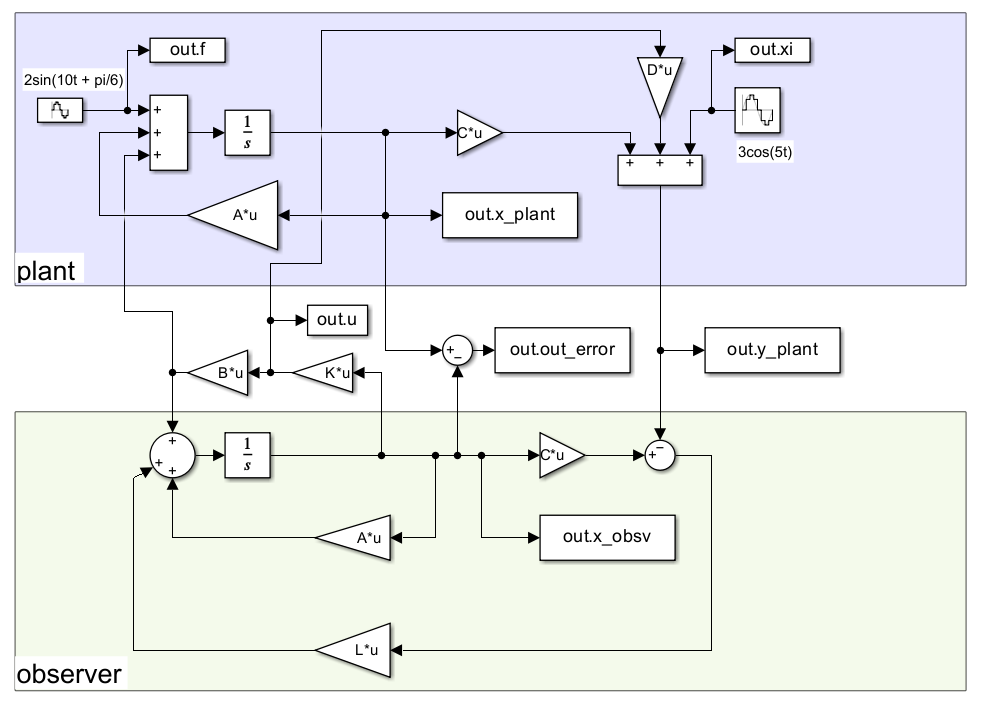
\includegraphics[width=0.8\textwidth]{model_observer_controlle_noise.png}
  \caption{Модель с LQD-регулятором-наблюдателем}
\end{figure}

В качестве детерминированных сигналов $f(t), \xi(t)$ возьмём следующие гармоники:
$$
  f(t) = 2sin(10t + \frac{\pi}{6}) , \tab \xi(t) = 3cos(5t)
$$

\subsection{Исследование управляемости системы}
Найдём собственные числа матрицы $A$:
$$
    \sigma(A) = \{-8, 4, 8, 16\}
$$
Воспользуемся прошлыми результатами - система будет полностью управляемой и наблюдаемой.

\newpage
\subsection{Синтез LQD}

Зададимся следующими парами матриц для регулятора $(Q_K, R_K)$ и наблюдателя $(Q_L, R_L)$:

$$
  Q_K = \begin{bmatrix}
    5 & 0 & 0 & 0 \\
    0 & 5 & 0 & 0 \\
    0 & 0 & 5 & 0 \\
    0 & 0 & 0 & 5 \\
\end{bmatrix}, \tab
R_K = \begin{bmatrix}
    20 & 0 \\
    0 & 20 \\
\end{bmatrix}
$$
$$
Q_L = \begin{bmatrix}
  1 & 0 & 0 & 0 \\
  0 & 1 & 0 & 0 \\
  0 & 0 & 1 & 0 \\
  0 & 0 & 0 & 1 \\
\end{bmatrix}, \tab
R_L = \begin{bmatrix}
  10 & 0 \\
  0 & 10 \\
\end{bmatrix}
$$
Теперь синтезируем регулятор и наблюдатель, используя решения матричных уравнений Риккати, которые упоминались в прошлых заданиях, 
здесь просто рамзерность повысится:
$$
  K = \begin{bmatrix}
    34.5 & -39.81 & 9.51 & 4.2 \\
    0 & 0 & 0 & 0 \\
\end{bmatrix}, \rightarrow \sigma(A+BK)=\{ -16.31, -8.5, -8, -6 \} 
$$
$$
  L = \begin{bmatrix}
    26.01 & -21.91 \\
    -29.19 & 13.58 \\
    -8.28 & 8.3 \\
    -11.46 & -0.03 \\
\end{bmatrix}, \rightarrow \sigma(A+LC)=\{ -16.01, -8.03, -8, -4 \}
$$

\newpage
\begin{figure}[ht]
  \centering
  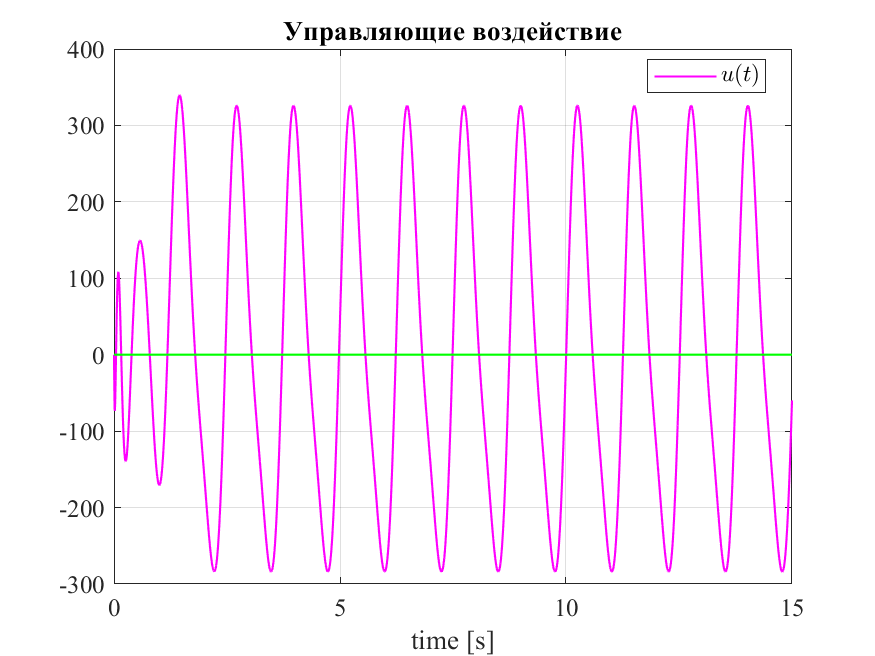
\includegraphics[width=0.8\textwidth]{lqg_u1.png}
  \caption{Сигнал управления}
\end{figure}
\begin{figure}[ht]
  \centering
  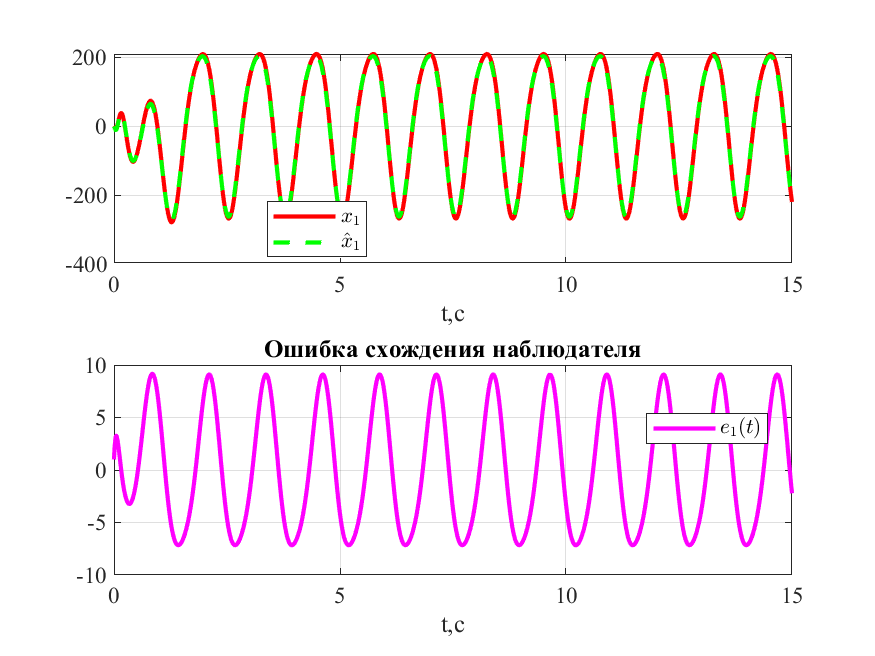
\includegraphics[width=0.8\textwidth]{lqg1.png}
  \caption{Состояние системы и наблюдатель}
\end{figure}
\newpage
\begin{figure}[ht]
  \centering
  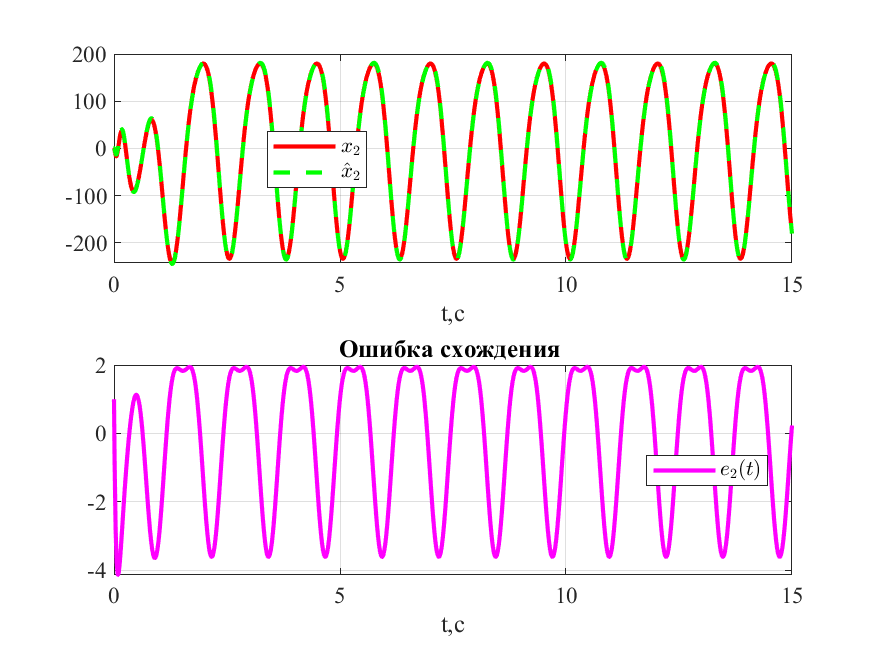
\includegraphics[width=0.8\textwidth]{lqg2.png}
  \caption{Состояние системы и наблюдатель }
\end{figure}
\begin{figure}[ht]
  \centering
  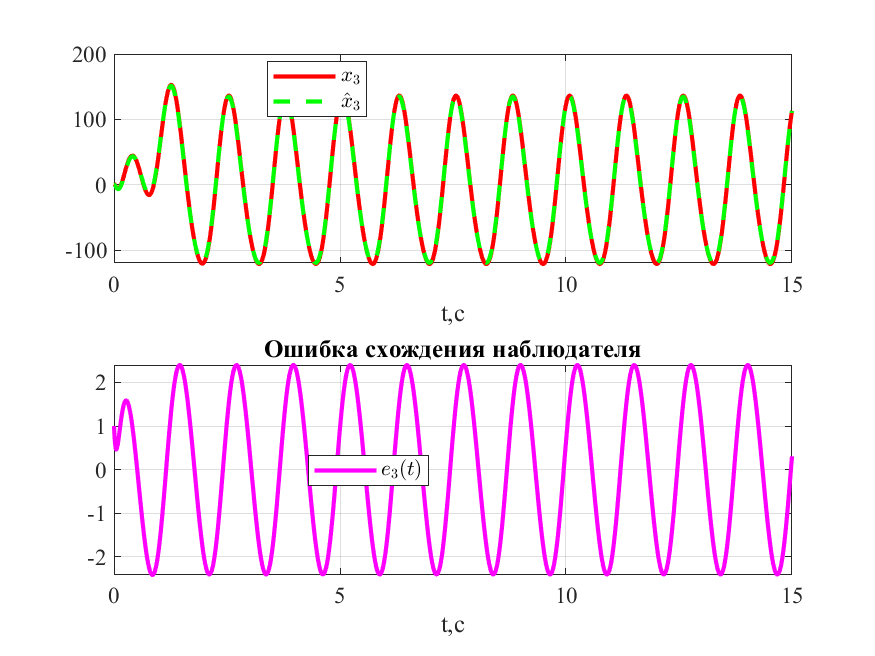
\includegraphics[width=0.8\textwidth]{lqg3.png}
  \caption{Состояние системы инаблюдатель}
\end{figure}
\newpage
\begin{figure}[ht]
  \centering
  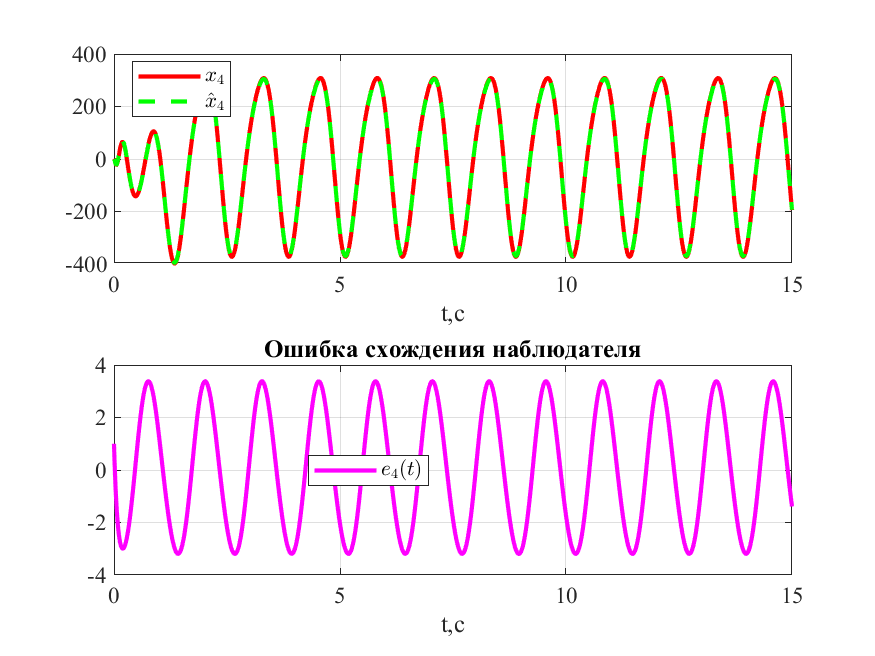
\includegraphics[width=0.8\textwidth]{lqg4.png}
  \caption{Состояние системы и наблюдатель}
\end{figure}

Можно заметить, что во всех случаях нам не удалось с помощью обозначенных параметров свести ошибку в ноль, это связано в том числе и с гармонической природой мешающих нам сигналов, 
мы не сможем свести их в ноль силами только П-регулятора, только лишь попробовать сделать амплитуду ошибки незначительно маленькой.

\subsection{Вывод}
В этом задании мы синтезировали \text{LQG = Linear Quadratic Gaussian} пару - регулятор и наблюдатель с использованием функционалов качества, они в целом отработали также, как и предполагалось: 
П-регулятора недостаточно для стабилизации гармонического типа сигнала, также повёл себя и наблюдатель, в курсе ЛСАУ для этого случая мы синтезировали специфичный регулятор.

\endinput